\documentclass[a4paper,10pt]{book}
\usepackage[utf8]{inputenc}

\usepackage[titletoc]{appendix}
\usepackage{graphicx}
\usepackage{float}
\usepackage{eso-pic}
\usepackage{anyfontsize}
\usepackage{multicol}
\usepackage{xcolor}
\definecolor{title}{RGB}{32,178,170}

\newenvironment*{chapterenv}{}{}
\newcommand\tab[1][0.5cm]{\hspace*{#1}}

\begin{document}
% Title Page
\begin{titlepage}
    \AddToShipoutPicture*{
    \AtPageUpperLeft{%
    \raisebox{-\height}{%
    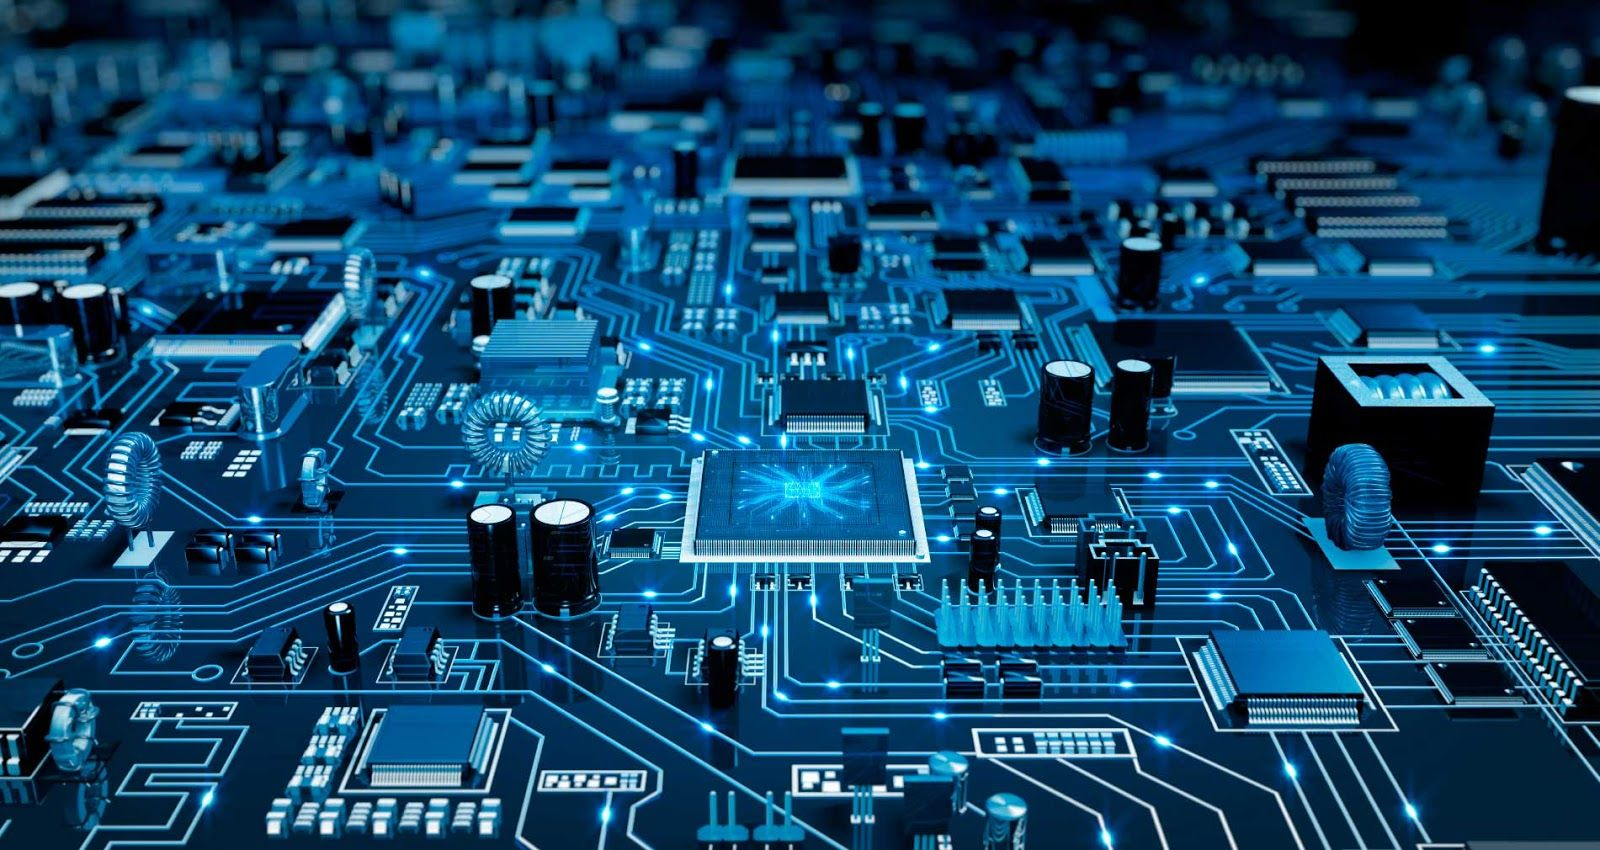
\includegraphics[width=\paperwidth,keepaspectratio]{./img/Title/title.jpg}
    }
    }
    };
    \vspace{7cm}
    \begin{center}
        {
        \fontsize{50}{60}\selectfont \textbf{ReapOnRoof}
        }
    \end{center}
    \begin{center}
        {
        \centering
        \fontsize{30}{50}\selectfont Electronic System Design Documentation
        }
    \end{center}
    
    \vspace{50px}
    
    \begin{center}
        \fontsize{30}{40} \textbf{Team}
    \end{center}
    
    \begin{center}
        \begin{multicols}{2}
            {
                \textbf{
                \fontsize{11}{13}\selectfont
                Aduri Sri Sambasiva Advaith\\
                email: evd18i002@iiitdm.ac.in\\
                phone: +91 85007 07368 \\
                \columnbreak
                Ajmeera Girish Kumar\\
                email: evd18i003@iiitdm.ac.in\\
                phone: +91 95731 02276
                }
            }
        \end{multicols}

    \end{center}


    
    \vspace{25px}
\end{titlepage}
{
    
    \begin{center}
        \vspace*{\fill}
        This page is left blank intentionally
        \vspace*{\fill}
    \end{center}
}

\tableofcontents

% Introduction
\begin{chapterenv}
    \chapter{Introduction}
    \textbf{ToDo}
\end{chapterenv}



\begin{appendices}
% List of Ideas
\begin{chapterenv}
    \chapter{List of Ideas}
    \section{Idea 1}
    \textbf{Idea}: Derivative of MQTT over Wired Connections(USB)\\
    \textbf{Explanation}:
    \newline
    \tab MQTT is an OASIS standard messaging protocol for IOT designed as an extremely lightweight publish/subscribe messaging transport for connecting devices using small code base and minimal bandwidth. An example MQTT architecture is given below:
    \begin{figure}[H]
    \centering
    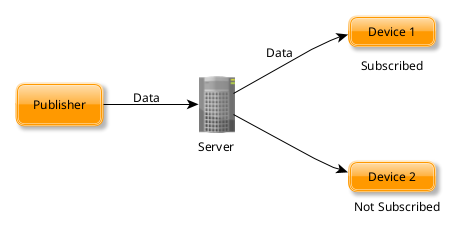
\includegraphics[width=0.75\textwidth,keepaspectratio=true]{img/Appendix A/I1/MQTT.png}
    % MQTT.bmp: 458x232 px, 183dpi, 6.36x3.22 cm, bb=0 0 180 91
    \end{figure}
    
    Here a publisher publishes a data which is sent to the server. Devices can subscribe to the publisher and the server sends data to the devices whenever the publisher sends some data. Those devices which does not subscribe to the publisher does not recieve the data as seen in the graph.
    \newline
    \tab In our system, we have sensors which detect external factors and send it to the server which then forwards it to actuators to take action. All the subsystems here communicate using wired protocols. Our idea is to develop a messaging protocol similar to MQTT to establish communication between sensors and actuators using wired communication.\\
    \textbf{Advantages}:
    \begin{itemize}
     \item Seperate sensors and actuators during pcb design allowing for better power supply design.
     \item Lightweight and Low Bandwidth
     \item Scaling is easy
    \end{itemize}
    \textbf{Work to be done}:
    \begin{itemize}
     \item Need to design a MQTT library for wired connection based on the protocol used.
     \item Provide support for different transmission speeds.
    \end{itemize}



\end{chapterenv}


\end{appendices}


\end{document}
